% !TEX options=--shell-escape
\documentclass [12pt]{article} 
\usepackage {amsmath}
\usepackage {amsthm}
\usepackage {amssymb}
\usepackage {graphicx} 
\usepackage {float}
\usepackage {multirow}
\usepackage {xcolor}
\usepackage {algorithmic}
\usepackage [ruled,vlined,commentsnumbered,titlenotnumbered]{algorithm2e} \usepackage {array} 
\usepackage {booktabs} 
\usepackage {url} 
\usepackage {parskip} 
\usepackage [margin=1in]{geometry} 
\usepackage [T1]{fontenc} 
\usepackage {cmbright} 
\usepackage [many]{tcolorbox} 
\usepackage [colorlinks = true,
            linkcolor = blue,
            urlcolor  = blue,
            citecolor = blue,
            anchorcolor = blue]{hyperref} 
\usepackage {enumitem} 
\usepackage {xparse} 
\usepackage {verbatim}
\usepackage{listings}
\usepackage{xcolor}
\usepackage{csquotes}
\usepackage[cache=false]{minted}
\usepackage{mdframed}
\usepackage{tikz}
\usetikzlibrary{shapes.symbols}
\newtheorem{theorem}{Theorem}

\DeclareTColorBox {Solution}{}{breakable, title={Solution}}
\DeclareTColorBox {Solution*}{}{breakable, title={Solution (provided)}}
\DeclareTColorBox {Instruction}{}{boxrule=0pt, boxsep=0pt, left=0.5em, right=0.5em, top=0.5em, bottom=0.5em, arc=0pt, toprule=1pt, bottomrule=1pt}
\DeclareDocumentCommand {\Expecting }{+m}{\textbf {[We are expecting:} #1\textbf {]}}
\DeclareDocumentCommand {\Points }{m}{\textbf {(#1 pt.)}} 
\newcommand {\hint }[1]{\noindent {[\textbf {HINT:} \em #1 \em ]}} \newcommand {\pts }[1]{\textbf {(#1 pt.)}} 

\begin{document} 

{\LARGE \textbf {COMP 285 (NC A\&T, Spr `22)}\hfill \textbf {Weekly Quiz 6} } 

\begin{Instruction}

\paragraph{Reporting Issues} If you find any issues with the solutions, reach out to Chi Wang (author) or Luis Perez (reviewer).

\end{Instruction}


\section{} Snakey the snake is in the bottom left corner of the grid, and is trying to reach O, the ultimate Oreo. 
Snakey can move from her current cell to the adjacent cells (right, left, up, or down) if they exist and are not marked with X (X cells are blocked). However, every time that Snakey moves from one cell to the other, Snakey has to eat a cookie. What is the minimum number of cookies Snakey needs to eat to get to the O? 

\begin{figure}[H]
    \centering
    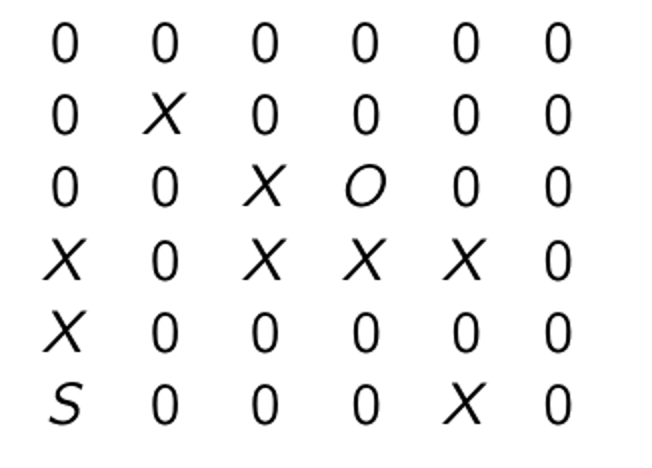
\includegraphics[scale=0.5]{6.png} 
    \label{fig:my_label}
\end{figure}

\begin{Solution}
10.
\paragraph{}
Shortest path problem. Go right, right, right, up, right, right, up, up, left, left.
\end{Solution}


\section{} Consider the general case of this problem, where a grid is given as an input with blocked and available cells and the locations of the Snakey and Oreo, and the goal is to find the minimum number of cookies for Snakey to reach the Oreo. Which algorithm would you use to solve this problem?

\begin{Solution}
BFS.
\end{Solution}


\section{} Assume you want to find the connected components of an undirected graph. Which algorithm would you use?

\begin{Solution}
BFS, DFS.
\end{Solution}


\section{} Consider the directed graph below. How many strongly connected components does this graph have?

\begin{figure}[H]
    \centering
    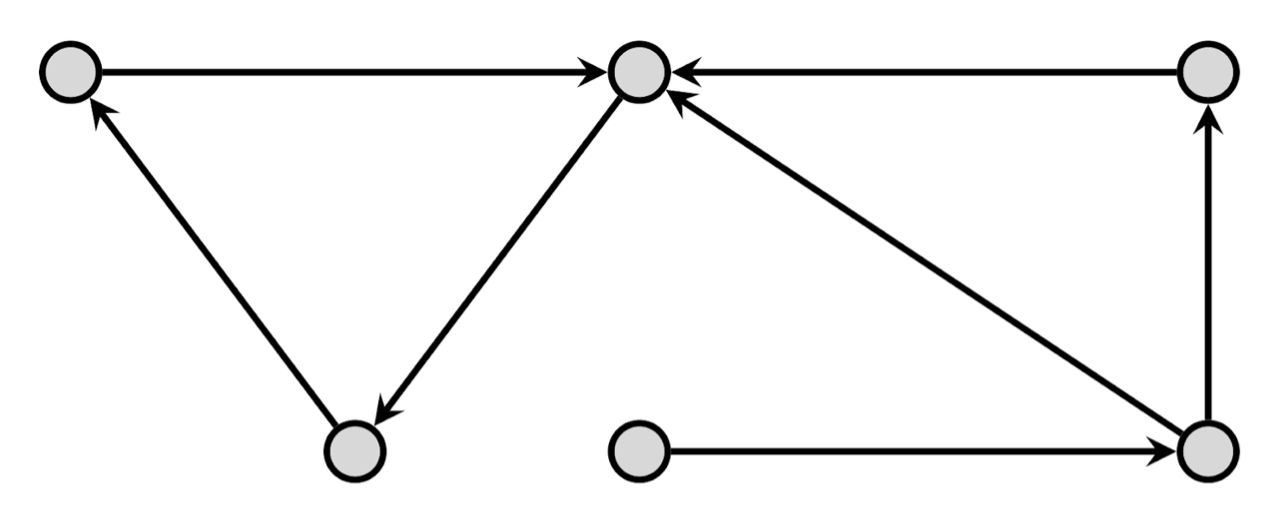
\includegraphics[scale=0.5]{2.png} 
    \label{fig:my_label}
\end{figure}

\begin{Solution}
4
\begin{figure}[H]
    \centering
    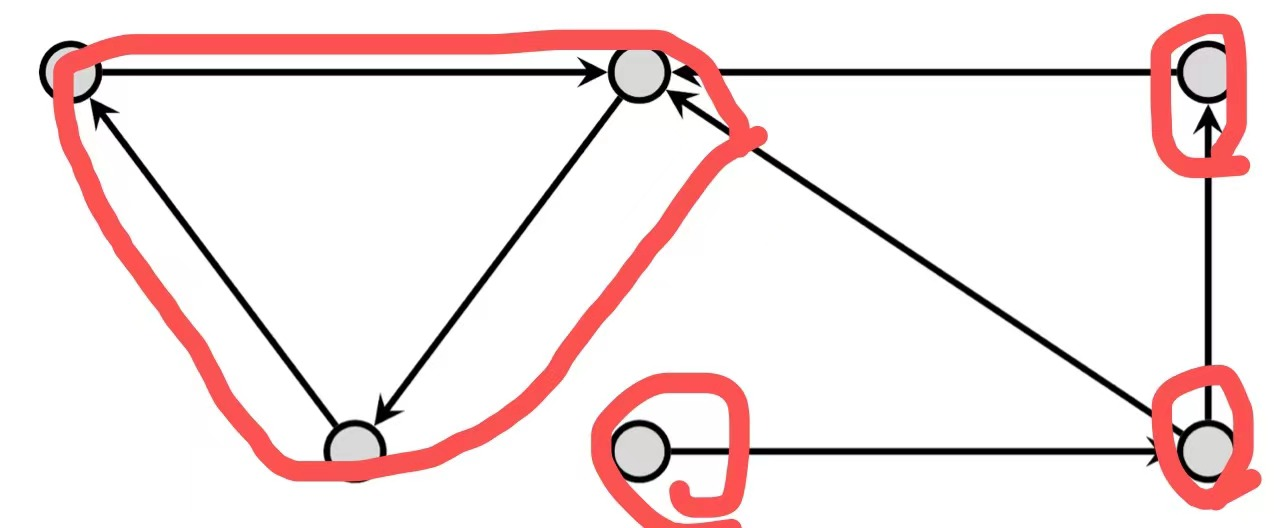
\includegraphics[scale=0.2]{4.jpeg} 
    \label{fig:my_label}
\end{figure}
\end{Solution}


\section{} Consider the directed graph below. What is the minimum number of directed edges to add to this graph to make all the vertices strongly connected? 
\begin{figure}[H]
    \centering
    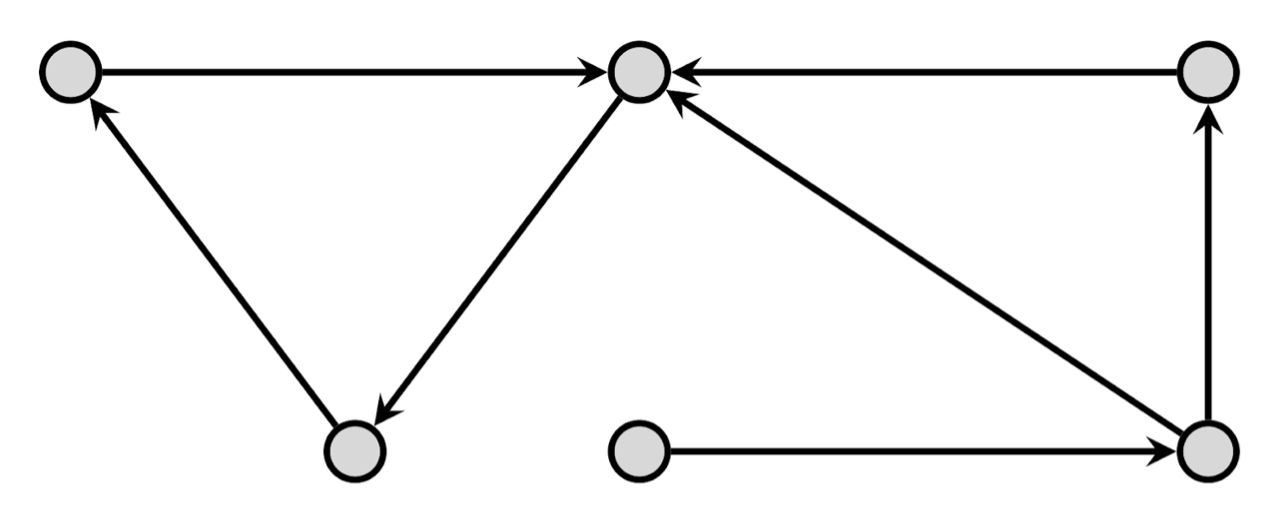
\includegraphics[scale=0.5]{2.png} 
    \label{fig:my_label}
\end{figure}

\begin{Solution}
1
\begin{figure}[H]
    \centering
    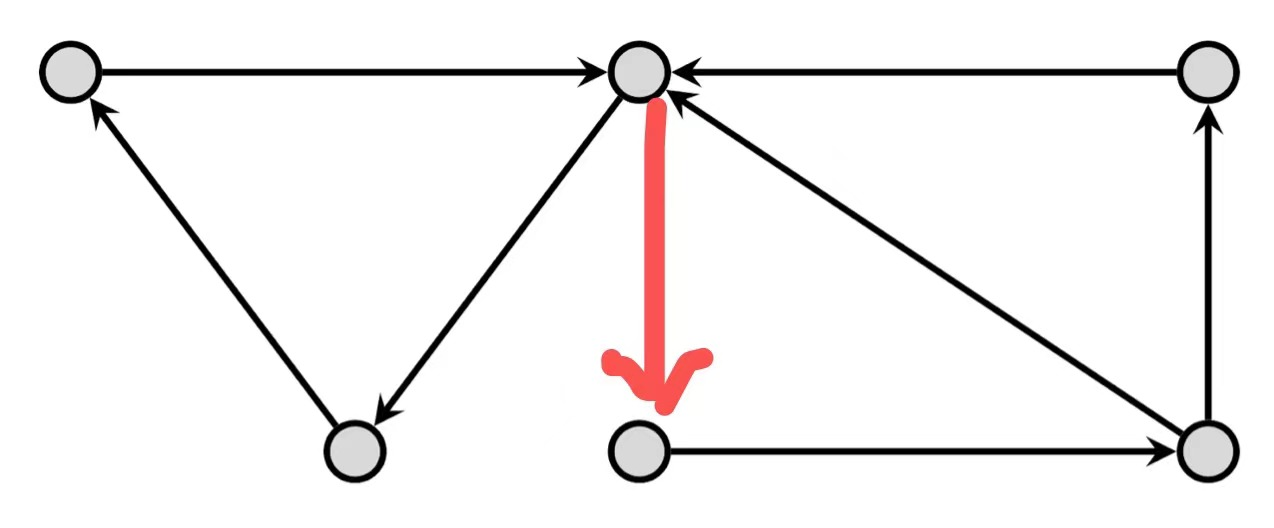
\includegraphics[scale=0.2]{5.jpeg} 
    \label{fig:my_label}
\end{figure}
\end{Solution}


\section{} Consider the Directed Acyclic Graph (DAG) below. Which of the below is a valid topological sorting of the graph?
\begin{figure}[H]
    \centering
    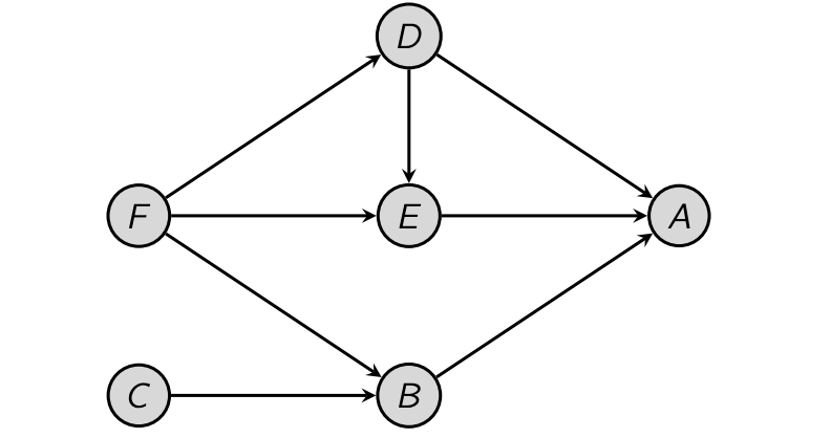
\includegraphics[scale=0.5]{3.png} 
    \label{fig:my_label}
\end{figure}

\begin{Solution}
FDCEBA
\end{Solution}


\section{} Consider the DAG below. What is the lexicographically smallest topological ordering of the vertices? There are many valid topological orderings - out of the valid ones, write the one where letters earlier in the alphabet appear first. To receive credit, enter your answer as capital letters with no spaces (eg, ABCDEF).
\begin{figure}[H]
    \centering
    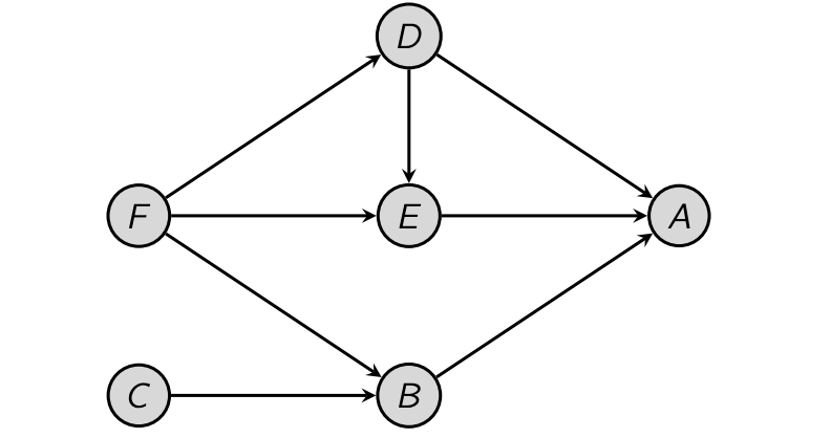
\includegraphics[scale=0.5]{3.png} 
    \label{fig:my_label}
\end{figure}

\begin{Solution}
CFBDEA
\end{Solution}


\section{} Assume you have two vertices u and v in a directed graph where u and v are in the same strongly connected components (SCC). Which one of the following is incorrect about u and v?
 
\begin{Solution}
There exists a DFS tree where u is not in v 's subtree and v is not in u's subtree.
\paragraph{}

A directed graph G = (V,E) is strongly connected if: 
for all $v, w$ in V: (1) there is a path from v to w and (2) there is a path from w to v.
So there couldn't exist such a DFS tree. 
\end{Solution}


\section{} Assume you have two vertices u and v in a directed graph where there exists a path from u to v. Which one of the following is incorrect about u and v?

\begin{Solution}
u's DFS finish time is always greater than v's DFS finish time.
\paragraph{}
It depends.
\end{Solution}



















\end{document} 